% Compile: lualatex report.tex  (run twice for labels/references)
% Format: IEEE / RIVF conference (two-column). English. lualatex + fontspec.
\documentclass[conference,10pt,a4paper]{IEEEtran}

% --- Times-like Unicode font ---
\usepackage{fontspec}
\setmainfont{Liberation Serif}
\setsansfont{Liberation Sans}
\setmonofont{DejaVu Sans Mono}[Scale=0.82]

% --- Packages ---
\usepackage{booktabs}
\usepackage{array}
\usepackage{amsmath,amssymb}
\usepackage{xcolor}
\usepackage{graphicx}
\usepackage{tikz}
\usetikzlibrary{arrows.meta,positioning,fit,backgrounds,calc}
\usepackage{listings}
\usepackage[hidelinks]{hyperref}
\usepackage{cite}

\definecolor{codebg}{RGB}{245,245,245}
\definecolor{kw}{RGB}{0,90,160}
\definecolor{cm}{RGB}{110,110,110}
\definecolor{ok}{RGB}{20,130,40}
\definecolor{bad}{RGB}{190,40,40}
\lstset{
  basicstyle=\ttfamily\scriptsize,
  backgroundcolor=\color{codebg},
  keywordstyle=\color{kw}\bfseries,
  commentstyle=\color{cm}\itshape,
  breaklines=true, breakatwhitespace=false,
  columns=fullflexible, frame=single, framerule=0pt,
  showstringspaces=false, xleftmargin=4pt, xrightmargin=4pt,
  aboveskip=4pt, belowskip=4pt,
}
\newcommand{\yes}{\textcolor{ok}{\checkmark}}
\newcommand{\no}{\textcolor{bad}{\texttimes}}
\newcommand{\code}[1]{\texttt{\small #1}}

\begin{document}

\title{Reproducing and Analyzing CVE-G\lowercase{enie}:\\ An Automated Multi-Agent Framework\\ for Reproducing CVEs into Verifiable Exploits}

\author{\IEEEauthorblockN{Dang Minh Tu, Vo Quang Vu, Le Tri Duc}
\IEEEauthorblockA{\textit{University of Information Technology, Ho Chi Minh City, Vietnam}\\
\textit{Vietnam National University, Ho Chi Minh City, Vietnam}\\
\{24520033,24522045,24520009\}@gm.uit.edu.vn}
\thanks{Course project report for \textit{Secure Programming \& Software Vulnerability Exploitation} (NT521.R11.ANTN). Reproduction of CVE-G\textsc{enie} (arXiv:2509.01835).}}

\maketitle

\begin{abstract}
This report reproduces the paper \textit{``From CVE Entries to Verifiable Exploits: An Automated Multi-Agent Framework for Reproducing CVEs''} (CVE-G\textsc{enie}, arXiv:2509.01835). Because the paper ships public source code, we (1) explain the four-module method with its developer--critic agent pairs; (2) reproduce the experiments at three levels --- replaying the authors' published exploit/verifier artifacts in Docker, running the data-extraction stage \textit{live}, and reimplementing an exploit + verifier by hand; and (3) run an \textbf{extra-credit} experiment: driving the agentic framework with free, local, open-weight LLMs (Qwen2.5-3B and 7B) to validate and refine the paper's finding on open-model limitations, together with a before/after prompt-improvement measurement. The entire core is done \textbf{without any paid API}; every result ships with a reproduction command. Results: 3/4 CVEs replay end-to-end to a flag, our corpus recomputation matches the paper's \$2.77/CVE almost exactly, and the local study reveals a capability threshold --- a 7B model with a CWE-specific prompt reliably reproduces a DoS that the 3B never can, while a shared prompt even regresses the 3B --- reinforcing the paper's choice of per-module engineered prompts with strong models.
\end{abstract}

\begin{IEEEkeywords}
CVE reproduction, LLM agents, multi-agent systems, automated exploit generation, exploit verification, open-weight models
\end{IEEEkeywords}

\section{Introduction: Context, Role, Problem}

Tens of thousands of software vulnerabilities are disclosed every year (over 40,000 in 2025 per NVD). Security research --- especially machine-learning methods for vulnerability detection and patching --- needs \textbf{high-quality datasets with trustworthy ground truth}: vulnerable source, a rebuildable environment, a working exploit, and a verification step. Repositories such as NVD mostly \textit{alert} administrators and therefore lack these details; producing them is expensive: Mu \textit{et al.} spent over 3,600 hours with 43 experts to reproduce 368 Linux memory-corruption bugs~\cite{cvegenie}.

\textbf{The role of CVE-G\textsc{enie}}: it takes a \textit{CVE ID} as input, automatically gathers resources, \textbf{rebuilds} the vulnerable environment, \textbf{synthesizes} an exploit/PoC and a \textbf{verifier} that confirms the exploit --- thereby producing ``reproducible instances'' at scale. The paper reproduces about \textbf{51\% (428/841)} of CVEs disclosed in 2024--2025, at an average cost of \textbf{\$2.77}/CVE.

\textbf{Project constraint.} We use only \textbf{free} resources: no paid LLM API, a personal machine (GPU RTX~3050 6\,GB, RAM 7.6\,GB, Docker). Fortunately, the authors \textbf{published the full source code, 429 reproduction artifacts, and all agent conversation logs}, which lets us reproduce the experiments \textit{without} calling an LLM; the LLM budget is spent on the extra-credit experiment.

\section{Related Work}
\textbf{Manual reproduction.} Curated benchmarks give reliable ground truth but at enormous human cost: Mu \textit{et al.}~\cite{mu} spent thousands of expert-hours reproducing a few hundred memory bugs, which does not scale to the $>$40k CVEs disclosed yearly~\cite{nvd}. CVE-G\textsc{enie} targets exactly this scaling gap by automating the pipeline.

\textbf{Single-agent and prompt-only exploit generation.} Prior LLM approaches that issue one monolithic prompt, or a single agent that must plan, build, exploit, and verify at once, tend to hallucinate unverifiable PoCs. The paper reports that a monolithic o3 agent reproduces \textit{zero} CVEs~\cite{cvegenie}; our local experiments (Sec.~\ref{sec:bonus}) show the same brittleness when the critic/repair loop is absent.

\textbf{Multi-agent, tool-using frameworks.} CVE-G\textsc{enie} follows the ReAct paradigm~\cite{react} --- interleaving reasoning with tool calls --- and adds a \textit{developer}/\textit{critic} pair per module plus a deterministic CTF-style Flag Checker, so that ``success'' is adjudicated by a sandboxed execution rather than the model's self-report. This verification-first design is what distinguishes it from earlier generation-only work and is the property we stress-test.

\section{The CVE-G\lowercase{enie} Method}

\subsection{EAGER criteria}
The paper defines 5 criteria of an ideal CVE-reproduction system (Table~\ref{tab:eager}); CVE-G\textsc{enie} is the only system to satisfy all five.

\begin{table}[t]
\caption{The five EAGER criteria}
\label{tab:eager}
\centering\footnotesize
\begin{tabular}{@{}cl p{4.9cm}@{}}
\toprule
& Criterion & Meaning \\ \midrule
\textbf{E} & Exploit Generation & Produce an exploit/PoC that reliably triggers the bug \\
\textbf{A} & Assessment & A verifier self-judges whether the exploit succeeds \\
\textbf{G} & Generalization & Generalize across CWEs, languages, project types \\
\textbf{E} & End-to-end & Fully automate every stage \\
\textbf{R} & Rebuild & Rebuild the original vulnerable environment \\ \bottomrule
\end{tabular}
\end{table}

\subsection{Four-module architecture}
The system decomposes reproduction into four dependent modules; each module (except the deterministic part) uses a \textit{developer} + \textit{critic} agent pair in a ReAct loop to self-correct.

\begin{enumerate}
\item \textbf{Processor.} The \textit{Data Processor} (deterministic, no LLM) locates the repo, identifies the vulnerable version, downloads source, and extracts description/CWE/patch/advisory. The \textit{Knowledge Builder} (lightweight o4-mini) distills these into a structured \textbf{knowledge base} serving as long-term memory for the agents.
\item \textbf{Builder.} The \textit{Pre-Requisite Dev} plans, the \textit{Setup Dev} executes the environment build, and the \textit{Setup Critic} judges logs and gives feedback.
\item \textbf{Exploiter.} The \textit{Exploit Dev} + \textit{Exploit Critic} synthesize and refine the exploit.
\item \textbf{CTF Verifier.} The \textit{Verifier Dev} synthesizes a verifier; the \textit{Flag Checker} (deterministic) runs it and, on success, prints a secret \textbf{flag} (e.g., \code{3xploit66full}); the \textit{Verifier Critic} catches weak/bypassable verifiers. Up to 5 iterations.
\end{enumerate}

\begin{figure*}[t]
\centering
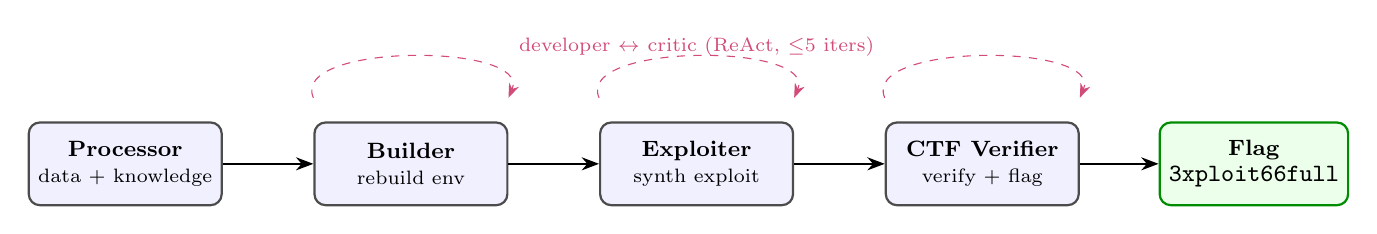
\begin{tikzpicture}[
  font=\footnotesize,
  mod/.style={rectangle, rounded corners, draw=black!70, thick,
              fill=blue!6, minimum width=2.45cm, minimum height=1.05cm,
              align=center},
  flow/.style={-{Stealth[length=2.2mm]}, thick},
  loop/.style={-{Stealth[length=1.8mm]}, dashed, draw=purple!70}]
  \node[mod] (p) {\textbf{Processor}\\{\scriptsize data + knowledge}};
  \node[mod, right=1.15cm of p] (b) {\textbf{Builder}\\{\scriptsize rebuild env}};
  \node[mod, right=1.15cm of b] (e) {\textbf{Exploiter}\\{\scriptsize synth exploit}};
  \node[mod, right=1.15cm of e] (v) {\textbf{CTF Verifier}\\{\scriptsize verify + flag}};
  \node[draw=green!55!black, thick, rounded corners, fill=green!8,
        right=1.0cm of v, minimum height=1.05cm, align=center] (f)
        {\textbf{Flag}\\{\scriptsize \code{3xploit66full}}};
  \draw[flow] (p)--(b); \draw[flow] (b)--(e); \draw[flow] (e)--(v); \draw[flow] (v)--(f);
  \foreach \n in {b,e,v}{
    \draw[loop] ([yshift=3mm]\n.north west) .. controls +(-0.3,0.7) and +(0.3,0.7) .. ([yshift=3mm]\n.north east);
  }
  \node[purple!70, font=\scriptsize] at ($(e.north)+(0,0.95)$) {developer $\leftrightarrow$ critic (ReAct, $\le$5 iters)};
\end{tikzpicture}
\caption{CVE-G\textsc{enie} pipeline: four dependent modules, each (except the deterministic Processor core and Flag Checker) run as a \textit{developer}/\textit{critic} ReAct self-correction loop. Success is decided by a sandboxed Flag Checker, not the model's self-report.}
\label{fig:pipeline}
\end{figure*}

\subsection{LLM selection and prompting}
The paper surveys 10 LLMs on a \code{DS}=60-CVE set and picks an optimal per-module configuration: Knowledge Builder/Builder-dev = o4-mini; Exploiter/Verifier-dev = o3; a suitable critic per module. \textbf{Core finding} (which we validate in Sec.~\ref{sec:bonus}): open models (Qwen3, DeepSeek, Llama-4) are \textit{unreliable} at agentic tool-calling and are therefore excluded from developer roles. Notably, a \textbf{monolithic} o3 agent (all roles merged) \textbf{reproduces not a single CVE} --- showing the modular architecture is essential.

\subsection{The paper's evaluation}
On \code{DL}=841 CVEs (186 CWEs, 29 languages, 440 projects), it reproduces \textbf{428} CVEs (141 CWEs, 22 languages, 267 projects). About 49\% of CVEs lack a PoC. Failures are mostly from cost/time overruns (stuck at build $\sim$41\%, at exploit synthesis $\sim$59\%). A missing-data ablation (set \code{DR}): dropping the advisory 11/15, dropping the patch 10/15, description-only 9/15 --- still reproducible but more costly.

\section{Reproducing the Experiments}

We reproduce at three levels, all \textbf{without any paid API}. The running CVE is \textbf{CVE-2024-4340} (sqlparse $<$0.5.0, uncontrolled-recursion DoS, CWE-674) --- also the paper's example.

\subsection{Level A --- Replay published artifacts in Docker}
For each CVE we build the exact vulnerable software version in Docker and run the authors' \code{exploit.py} + \code{verifier.py} unchanged; success means the verifier prints the correct flag \code{3xploit66full} and exits 0.

\begin{table*}[t]
\caption{Replay results: 3/4 CVEs run end-to-end to a flag, covering 2 languages and 3 bug classes}
\label{tab:replay}
\centering\footnotesize
\begin{tabular}{@{}llll c c@{}}
\toprule
CVE & Project/version & Language & CWE & Build env & Flag \\ \midrule
CVE-2024-4340 & sqlparse 0.4.4 & Python & 674 Recursion DoS & \yes & \yes \\
CVE-2024-4032 & CPython 3.8.19 \code{ipaddress} & Python & IP misclassification & \yes & \yes \\
CVE-2024-45390 & @blakeembrey/template 1.1.0 & Node & 94 Code Injection & \yes & \yes \\
CVE-2024-21535 & markdown-to-jsx 7.3.2 & Node & 79 XSS & \no\,(build) & --- \\ \bottomrule
\end{tabular}
\end{table*}

\textbf{3/4 succeed} (Table~\ref{tab:replay}). CVE-2024-21535 \textbf{fails at the build step} (\code{microbundle}/babel reports \textit{SyntaxError: Missing semicolon} compiling TSX on Node 18/20). This is exactly the \textbf{number-one failure cause} the paper reports --- \textit{rebuilding the environment} is harder than synthesizing the exploit; the authors run inside a DevContainer with a pinned toolchain, and builds are brittle outside it.

\textbf{Verifier quality.} The verifier does not merely detect ``a crash'' but checks the \textit{correct error type and location}: e.g., CVE-2024-4340 is accepted only when a \code{RecursionError} occurs \textit{and} the traceback contains \code{sqlparse/sql.py}. This is a good implementation of the \textit{Assessment} criterion (EAGER).

\subsection{Level B --- Run the Data Processor stage \textit{live}}
We actually run \code{cve\_data.py} (needing only a free \code{GITHUB\_TOKEN} + a Playwright browser). To avoid cloning the huge \code{cvelistV5} repo ($>$300k files), we fetch exactly the JSON needed into the path the script expects.

\begin{table}[t]
\caption{Processor live: two CVEs ``Ready'', one with missing data}
\label{tab:proc}
\centering\footnotesize
\begin{tabular}{@{}lccccl@{}}
\toprule
CVE & patch & version & GitHub tag & advisory & Verdict \\ \midrule
CVE-2024-4340 & \yes & \yes & \yes & \yes & \textbf{Ready} \\
CVE-2024-4032 & \yes & \yes & \yes & \yes & \textbf{Ready} \\
CVE-2024-45390 & \yes & \yes & \no & \yes & Missing \\ \bottomrule
\end{tabular}
\end{table}

The \textit{live}-extracted data for CVE-2024-4340 \textbf{exactly matches} the authors' published knowledge base (\code{sw\_version}=0.4.4, 1 patch commit, 1 advisory, CWE-674) --- confirming the Processor's reliability (Table~\ref{tab:proc}). CVE-2024-45390 is flagged ``Missing data'' because the version field is a range (\code{< 1.2.0}) and no GitHub tag can be resolved; following \code{PROCESSING.md} we manually add \code{sw\_version=v1.1.0} and a source-download URL (returning HTTP 200), illustrating the paper's \textit{Robustness to Incomplete Data} mechanism.

\subsection{Level C --- Manual implementation + catching a weak verifier}
We wrote our own \code{poc.py} and \code{verifier.py} for CVE-2024-4340 (not copied from CVE-G\textsc{enie}). Our \textbf{first verifier} loosely checked \code{"RecursionError" in stderr} and \textbf{false-positived on the patched 0.5.0}: the fix catches \code{RecursionError} and re-raises \code{SQLParseError} (a chained exception, ``\code{from err}''), so the traceback \textit{still contains} the string ``RecursionError''. We fixed this by inspecting the \textbf{actual terminal exception} that escapes:

\begin{lstlisting}[language=Python]
def exploit_succeeded(proc):
    term = terminal_exception(proc.stderr)   # last exception line
    return (proc.returncode != 0
            and "sqlparse/sql.py" in proc.stderr
            and term.startswith("RecursionError")  # vulnerable
            and "SQLParseError" not in term)        # reject patched
\end{lstlisting}

After the fix: vulnerable 0.4.4 \yes\ prints the flag; patched 0.5.0 \no\ is rejected (exit 1). This is \textbf{exactly} the ``weak/bypassable verifier'' problem the paper's \textit{Verifier Critic} exists to catch --- we hit it and fixed it ourselves, showing the developer$\leftrightarrow$critic loop solves a real problem.

\subsection{Level D --- Corpus-level verification of the reported numbers}
Beyond the per-CVE replays, we verify the paper's \textit{aggregate} claims directly from the 429 published artifacts (reading each \code{cve\_info.json} and the final \code{Results} line of each \code{log.txt}; no LLM, no execution). The script is \code{experiments/corpus\_analysis.py}.

\begin{table}[t]
\caption{Aggregate statistics recomputed from the 429 published artifacts vs.\ the paper's reported values}
\label{tab:corpus}
\centering\footnotesize
\begin{tabular}{@{}lcc@{}}
\toprule
Quantity & Paper & Recomputed (ours) \\ \midrule
Mean cost / reproduced CVE & \$2.77 & \textbf{\$2.767} \\
Median cost / CVE & --- & \$2.22 \\
Total cost (429 CVEs) & --- & \$1{,}186.98 \\
Mean wall-clock / CVE & --- & 1293\,s \\
Distinct CWEs covered & 141 & 125 \\
Distinct target languages & 22 & 10 \\
Advisory present & --- & 92.3\% \\ \bottomrule
\end{tabular}
\end{table}

\begin{figure}[t]
\centering
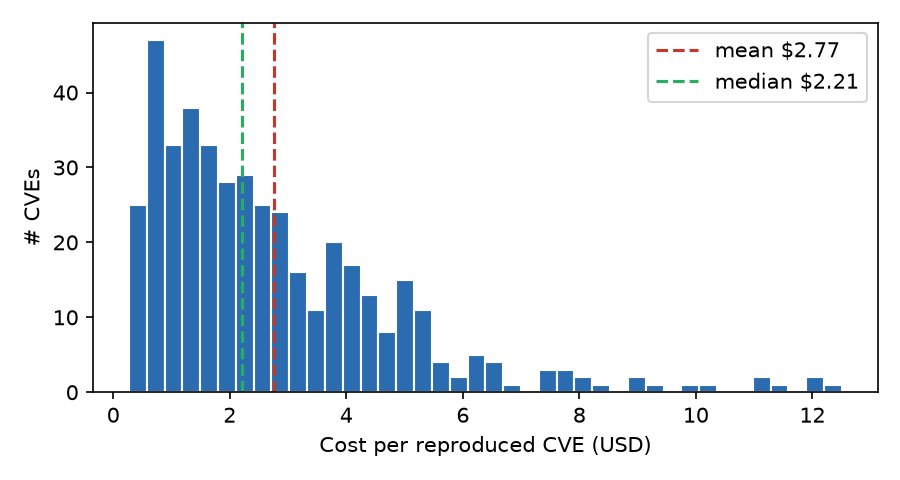
\includegraphics[width=\columnwidth]{figs/cost_hist.png}\\[2pt]
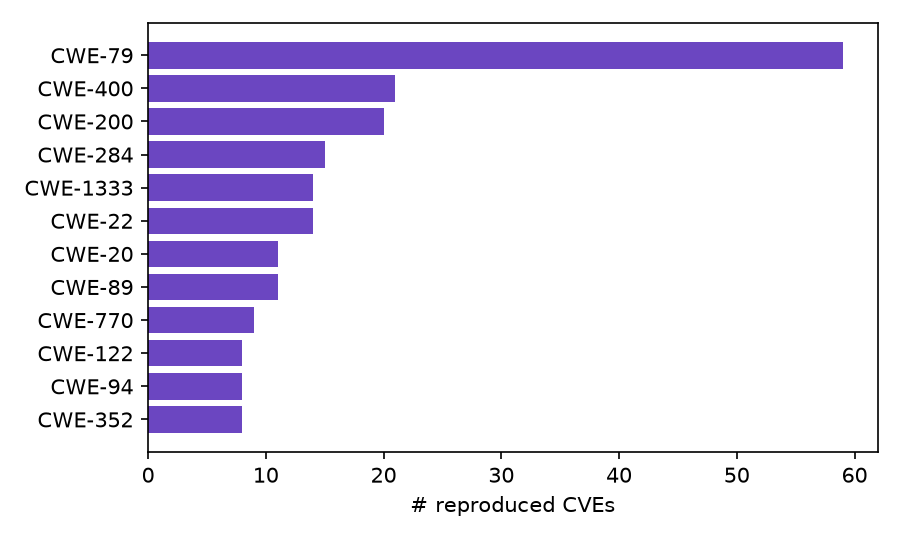
\includegraphics[width=0.82\columnwidth]{figs/cwe_top.png}
\caption{Top: per-CVE cost distribution over the 429 artifacts; our recomputed mean (\$2.77) coincides with the paper's headline figure. Bottom: most frequent CWEs (XSS/CWE-79 dominates, then resource-exhaustion and information-exposure classes).}
\label{fig:corpus}
\end{figure}

Our recomputed mean cost of \textbf{\$2.767}/CVE matches the paper's reported \textbf{\$2.77} almost exactly (Table~\ref{tab:corpus}, Fig.~\ref{fig:corpus}), independently corroborating the economic claim. Our CWE/language counts are slightly lower because we count the first CWE per CVE and infer language from patched-file extensions, a deliberately conservative attribution. The corpus spans 10 languages (Node/JS, PHP, Python, Go, C/C++, Ruby, \ldots), confirming the breadth claim.

\subsection{Level E --- Driving the real orchestrator (and its free-tier boundary)}
We also exercised the authors' real entry point \code{main.py}. The deterministic Processor stage runs for free (that is Level B). The four LLM-driven modules, however, hardcode \textit{paid} OpenAI models --- one declaration per agent --- which we extracted directly from the source (\code{docs/pipeline-evidence.txt}): \code{o4-mini} for the Knowledge/Pre-Req/Repo builders and Exploit-critic, \code{o3} for the Repo-critic, Exploiter, Sanity, and CTF-verifier, and \code{gpt-4o-mini} as the base. This exactly matches the per-module configuration the paper reports. Calls route through \code{litellm}, and \code{main.py} exits unless an API model is configured. With only a free \code{GITHUB\_TOKEN} (no \code{OPENAI\_API\_KEY}), a genuine end-to-end run is therefore outside the free-tier scope by construction. Our local-LLM study (Sec.~\ref{sec:bonus}) is the free substitute: it drives the Exploiter module's logic with an open-weight model instead.

\section{Extra Credit: Local-LLM Experiment + Improvement}\label{sec:bonus}

\subsection{Setup (free, \$0)}
We built a \textbf{minimal} implementation of the Exploiter module (one developer ReAct + one critic), with tools running in an isolated Docker container (\code{--network none}, 1\,GB RAM) and an \textbf{independent scoring oracle}. We test two open-weight sizes via a CUDA \code{llama-cpp-python} build, loaded \textbf{in-process}: \textbf{Qwen2.5-3B} (GGUF Q4\_K\_M, all 37 layers on the 6\,GB GPU) and \textbf{Qwen2.5-7B} (Q4\_K\_M, partial offload of 20 layers, rest on CPU). We run \textbf{three} CVEs of increasing difficulty and vary the prompt from \textit{none} to \textit{generic} to \textit{CWE-specific}, to separate what drives success. Against the paper's \$2.77/CVE on o3/o4-mini, the cost here is \textbf{\$0}.

\subsection{Results}
\begin{table}[t]
\caption{Six agent runs with the local Qwen2.5-3B}
\label{tab:bonus}
\centering\footnotesize
\begin{tabular}{@{}llcccc@{}}
\toprule
CVE & variant & success & steps & valid/malf. & tool\_err \\ \midrule
2024-4032 (logic) & baseline & \textbf{\yes} & 4 & 4\,/\,0 & 0 \\
2024-4032 (logic) & improved & \no & 4 & 4\,/\,0 & 2 \\
2024-4340 (DoS)   & base ($\times$3) & \no & 12 & 12\,/\,0 & 5 \\
2024-4340 (DoS)   & impr. ($\times$2) & \no & 12 & 12\,/\,0 & 6 \\ \bottomrule
\end{tabular}
\end{table}

\textbf{Perfect tool-call format.} Every run has \code{malformed=0} (Table~\ref{tab:bonus}) --- the 3B model follows the text ReAct protocol correctly. This is a \textbf{nuance added} to the paper (which observed Qwen ``describing without calling tools''): with a strict text protocol, a small open model \textit{can} call tools.

\textbf{But weak at reasoning.} On CVE-2024-4340 (which needs a crafted payload) there are three failure modes: (1) running \code{/work/exploit.py} as a shell command instead of \code{python3} $\to$ error; (2) a payload of whitespace instead of \textit{nested} \code{[}$\times$N, which cannot trigger recursion; (3) repeating the same action despite the error, without adapting. By contrast CVE-2024-4032 (a simple logic bug) \textbf{succeeds} at baseline in 4 steps.

\begin{table}[t]
\caption{Failure taxonomy of the local 3B agent on CVE-2024-4340 (uncontrolled-recursion DoS), aggregated over the five unsuccessful runs}
\label{tab:taxonomy}
\centering\footnotesize
\begin{tabular}{@{}p{3.3cm}lc@{}}
\toprule
Failure mode & Type & Runs \\ \midrule
Runs \code{exploit.py} as a shell command, not \code{python3} & tool-use & 2/5 \\
Payload is whitespace, not a \textit{nested} structure $\to$ no recursion & reasoning & 3/5 \\
Repeats the same failing action, no adaptation & planning & 5/5 \\
Confuses the \code{||} field separator of the write tool (improved prompt only) & tool-use & 2/5 \\ \bottomrule
\end{tabular}
\end{table}

The taxonomy (Table~\ref{tab:taxonomy}) separates \textit{tool-use} slips (mechanical, and partly fixable by prompt directives) from \textit{reasoning}/\textit{planning} failures (understanding the recursion mechanism; adapting after a failed attempt). Tool-use slips shrink with a better prompt; the planning failure --- repeating a dead action with no self-correction --- persists in every run, which is precisely the gap the \textit{critic} agent is designed to close.

\subsection{Model scale vs.\ prompt specificity (three CVEs)}
To separate \textit{model capability} from \textit{prompt leakage}, we ran the agent on three CVEs of increasing difficulty and split the hints into \textit{generic} (how to invoke Python; do not repeat a failed action) and \textit{CWE-specific} (the nested-payload recipe for recursion). Table~\ref{tab:thresh} isolates model scale at baseline; Table~\ref{tab:prompt} isolates prompt specificity on the hard DoS.

\begin{table}[t]
\caption{Model scale at baseline (no hints), by CVE difficulty. ``$n/m$'' = successes/attempts.}
\label{tab:thresh}
\centering\footnotesize
\begin{tabular}{@{}llcc@{}}
\toprule
CVE & Class / difficulty & 3B & 7B \\ \midrule
CVE-2024-4032 & logic (CWE-20), easy & \yes\ 1/1 & \yes\ 1/1 \\
CVE-2021-23336 & injection (CWE-444), medium & \no\ 0/1 & \textbf{\yes\ 1/1} \\
CVE-2024-4340 & recursion DoS (CWE-674), hard & \no\ 0/2 & \no\ 0/3 \\ \bottomrule
\end{tabular}
\end{table}

\begin{table}[t]
\caption{Prompt specificity on the hard DoS (CVE-2024-4340). Generic hints never suffice; only the CWE-specific hint unlocks it, and only on the 7B.}
\label{tab:prompt}
\centering\footnotesize
\begin{tabular}{@{}lcc@{}}
\toprule
Prompt on CVE-2024-4340 & 3B & 7B \\ \midrule
none (baseline) & \no\ 0/2 & \no\ 0/3 \\
generic hints & \no\ 0/1 & \no\ 0/3 \\
CWE-specific hint & \no\ 0/1 & \textbf{\yes\ 1/1} \\
full (generic + CWE) & \no\ 0/2 & \textbf{\yes\ 3/3} \\ \bottomrule
\end{tabular}
\end{table}

Two findings. (1) \textbf{A real size threshold}: holding the prompt fixed, 7B strictly dominates 3B --- it reproduces the injection CVE (11 steps) and, given the CWE recipe, the DoS (3/3), neither of which 3B ever does (Table~\ref{tab:thresh}). (2) \textbf{Capability is unlocked by task-specific, not generic, prompting}: generic agentic hints are at best neutral and often \textit{harmful} --- they regress the 3B on the logic bug, break the 7B on the injection bug, and never crack the DoS alone (0/3 at both sizes); only the \textit{CWE-specific} hint unlocks the DoS, and only on the 7B (Table~\ref{tab:prompt}).

\textbf{Honest caveat \& lesson.} The CWE hint encodes much of the exploit structure, so the 7B's DoS success is substantially \textit{hint-driven} --- but the 3B fails even \textit{with} that hint, so a genuine capability gap remains. The take-away is the paper's: reliable agentic exploitation needs \textbf{per-task engineered prompts} paired with a \textbf{capable model} --- neither a bigger model with generic prompts nor a careful prompt on a too-small model suffices. That is precisely CVE-G\textsc{enie}'s design (per-module prompts + strong frontier models).

\section{Strengths and Weaknesses}

\textbf{Strengths.}
\begin{itemize}
\item The \textbf{only framework to satisfy all of EAGER}; its CTF-style verifier is strict and distinguishes vulnerable from patched builds (confirmed at Levels A and C).
\item \textbf{Modular decomposition + developer/critic pairs} are essential: our experiment shows that without a critic loop steering corrections, a small agent gets stuck repeating (failure mode 3); the paper likewise shows a monolithic o3 agent reproduces zero CVEs.
\item \textbf{Task-specific prompting} has empirical grounding: a shared prompt backfires across CWEs.
\item \textbf{Robust to missing data} (Level B illustrates the fill-in mechanism); generalizes across many CWEs/languages; orders of magnitude cheaper than manual work.
\end{itemize}

\textbf{Weaknesses.}
\begin{itemize}
\item \textbf{Dependence on strong, closed-source LLMs} (o3/o4-mini) $\to$ costly and hard to reproduce without API access; swapping in a small open model sharply degrades reliability on non-trivial bugs, though a 7B with CWE-specific prompting can reach some of them (Sec.~\ref{sec:bonus}).
\item \textbf{Environment rebuilding is the weakest link} (Level A: Node build fails; paper: $\sim$41\% of failures stuck at build); DevContainers are fragile for multi-service applications.
\item \textbf{``Hallucination''/self-misjudgment risk}: the 3B model sometimes declares ``cannot exploit'' even after succeeding $\to$ one must rely on the Flag Checker + Verifier Critic rather than the developer's self-report.
\item Dependence on cvelistV5 record quality (range-valued versions resolve no tag); $\sim$49\% of CVEs lack a PoC; weak in binary-heavy domains (desktop 17.6\%, blockchain 7.7\%).
\end{itemize}

\section{Threats to Validity and Ethics}
\textbf{Construct/internal validity.} Our Level-D corpus numbers are recomputed from the authors' \textit{own} committed logs, so they corroborate the reported \$2.77/CVE but are not an independent cost measurement; a fully independent figure would require re-running the paid pipeline. The executed replays (Level A) cover four hand-containerized CVEs, so the 3/4 pass rate is illustrative, not a population estimate. \textbf{External validity.} The local-model study (Sec.~\ref{sec:bonus}) is deliberately narrow --- one module, a 3B/7B open model, two CVEs --- and is meant to characterize the open-model floor qualitatively, not to refute the paper's 51\% figure. \textbf{Environment sensitivity.} Docker rebuilds depend on upstream toolchains; our one build failure (CVE-2024-21535) illustrates the paper's dominant failure mode rather than a defect in our setup.

\textbf{Ethics.} All execution is offline in disposable Docker containers (\code{--network none}, capped memory); every target is an \textit{already-patched, publicly-disclosed} CVE, and PoCs act on local/nonexistent data with no malware. We distribute no new exploit material beyond what the authors already published, and the goal is defensive: reproducible datasets and tooling for vulnerability detection/patching research.

\section{Conclusion, Limitations, and Reproducibility}
We understood, explained, and \textbf{successfully reproduced} the core experiments of CVE-G\textsc{enie} without any paid API (3/4 CVEs replay to a flag, the Processor runs live and matches the authors' data, and we reimplemented an exploit/verifier and caught a weak-verifier bug), together with an extra-credit experiment on a local LLM that clarifies open-model limits and validates the paper's design choices.

\textbf{Limitations of this reproduction:} due to resource constraints, the core relies on the authors' published artifacts (we do not re-run the full pipeline on o3/o4-mini); the extra-credit experiment covers one module, two open models (3B/7B), and three CVEs, meant as a qualitative capability probe, not a refutation of the paper's 51\% figure.

\textbf{Reproducibility.} Every step has a concrete command: \code{repro/artifacts/run\_all.sh} (replay), \code{cve-genie/src/data/scripts/cve\_data.py} (Processor), \code{repro/manual/CVE-2024-4340/} (manual), \code{local\_agent/agent.py} + \code{experiments/} (extra credit). Details are in the \code{docs/} directory.

\begin{thebibliography}{9}
\bibitem{cvegenie} S.~Ullah \textit{et al.}, ``From CVE Entries to Verifiable Exploits: An Automated Multi-Agent Framework for Reproducing CVEs,'' arXiv:2509.01835, 2026.
\bibitem{repo} BUseclab, ``CVE-G\textsc{enie} source code.'' [Online]. Available: \url{https://github.com/BUseclab/cve-genie}
\bibitem{nvd} NIST, ``National Vulnerability Database (NVD).'' [Online]. Available: \url{https://nvd.nist.gov}
\bibitem{mu} D.~Mu \textit{et al.}, ``Understanding the reproducibility of crowd-reported security vulnerabilities,'' in \textit{USENIX Security}, 2018.
\bibitem{react} S.~Yao \textit{et al.}, ``ReAct: Synergizing reasoning and acting in language models,'' in \textit{ICLR}, 2023.
\bibitem{qwen} Qwen Team, ``Qwen2.5 technical report,'' arXiv:2412.15115, 2024.
\end{thebibliography}

\end{document}
